\chapter{Methods}

\section{Lusia Violita Aprilian/1164080}
\subsection{Teori}
\begin{enumerate}
\item Random Forest
	\begin{itemize}
	\item Random Forest diperkenalkan dan diselidiki untuk memprediksi aktivitas biologis kategoris atau kategoris suatu senyawa berdasarkan pada deskripsi kuantitatif dari struktur molekul senyawa. Random Forest adalah ensemble dari pohon klasifikasi atau regresi yang tidak ditandai yang dibuat dengan menggunakan sampel bootstrap dari data pelatihan dan pemilihan fitur acak dalam induksi pohon. Prediksi dibuat dengan menggabungkan (suara terbanyak atau rata-rata) prediksi ensemble.
	\item Gambar Random Forest
		\begin{figure}[ht]
		\centering
		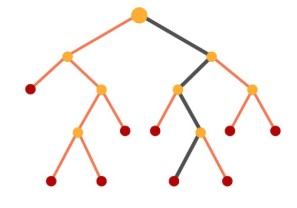
\includegraphics[scale=0.5]{figures/j1.jpg}
		\caption{Random Forest}
		\label{contoh}
		\end{figure}
	\end{itemize}

\item Membaca Dataset
	\begin{itemize}
	\item Berikut adalah cara membaca dataset :
		\begin{enumerate}
			\item Buka Anaconda Navigator lalu jalankan Syper, kemudian import libraries yang dibutuhkan.
			\item Masukkan kode python untuk membaca file csv, lalu jalankan.
				\begin{figure}[ht]
				\centering
				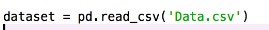
\includegraphics[scale=0.8]{figures/j41.jpg}
				\caption{Kode Python}
				\label{contoh}
				\end{figure}
			\item Maka pada window console akan menampilkan pesan berikut :
				\begin{figure}[ht]
				\centering
				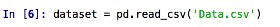
\includegraphics[scale=0.9]{figures/j42.jpg}
				\caption{Pesan Window Console}
				\label{contoh}
				\end{figure}
			\item Dari explorer dapat terlihat dataset yang terimport.
				\begin{figure}[ht]
				\centering
				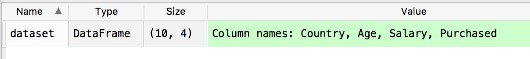
\includegraphics[scale=0.6]{figures/j43.jpg}
				\caption{Dataset}
				\label{contoh}
				\end{figure}
			\item Lalu klik dataset cell, maka akan muncul seperti berikut :
				\begin{figure}[ht]
				\centering
				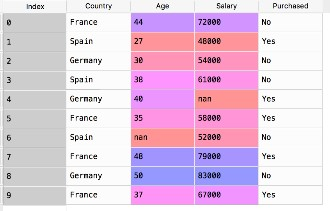
\includegraphics[scale=0.7]{figures/j44.jpg}
				\caption{Hasil Dataset Cell}
				\label{contoh}
				\end{figure}
			\item Seperti yang terlihat pada gambar tersebut dataset ini memiliki Kolom Country, Age, dan Salary sebagai independent variable-nya dan kolom Purchased sebagai dependent variable-nya.
			\item Selanjutnya buat 2 matrix of features yang berisi values dari independent variable dan dependent variable.
			\item Lalu tuliskan perintah berikut :
				\begin{figure}[ht]
				\centering
				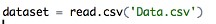
\includegraphics[scale=0.9]{figures/j45.jpg}
				\caption{Perintah}
				\label{contoh}
				\end{figure}
			\item Perintah yang telah dibuat di atas akan membuat sebuah global environment baru dan muncul dataset.
			\item Klikdataset tersebut maka muncul tabel berisi dataset.
		\end{enumerate}
	\end{itemize}

\item Cross Validation
	\begin{itemize}
		\item Cross validation adalah metode statistik yang digunakan untuk memperkirakan keterampilan model pembelajaran mesin. Ini biasanya digunakan dalam pembelajaran mesin yang diterapkan untuk membandingkan dan memilih model untuk masalah pemodelan prediktif yang diberikan karena mudah dipahami, mudah diimplementasikan, dan menghasilkan estimasi keterampilan yang umumnya memiliki bias lebih rendah daripada metode lainnya.
	\end{itemize}
	
\item Menjelaskan Arti Score
	\begin{itemize}
		\item Maksud arti score 44\% pada random forest adalah hasil akurasi.
		\item Maksud arti score 27\% pada decission tree adalah presentasi hasil dari perhitungan dataset.
		\item Maksud arti score 29\% dari SVM adalah hasil pendekatan neural network.
		\item Hasil tersebut didapat dari hasil valdasi silang untuk memastikan bahwa membagi  training test dengan cara yang berbeda. Sehingga didapat outputnya 44\% untuk hutan acak, 27\% untuk pohon keputusan, dan 29\% untuk SVM.
	\end{itemize}

\item Cara Membaca Confusion Matriks
	\begin{itemize}
		\item Mari kita lihat contoh klasifikasi biner berikut ini, yang menunjukkan berapa kali model telah membuat prediksi objek yang benar:
			\begin{figure}[ht]
			\centering
			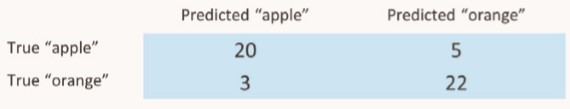
\includegraphics[scale=0.5]{figures/j2a.jpg}
			\caption{Tabel Confusion Matriks}
			\label{contoh}
			\end{figure}
		\item Dalam tabel tersebut, baris apple dan orange mengacu pada kasus di mana objek tersebut sebenarnya sebuah apel atau sebuah jeruk. Kolom merujuk pada prediksi yang dibuat oleh model. Kita melihat bahwa dalam contoh ada 20 apel yang diprediksi dengan benar, sementara ada 5 apel yang salah diidentifikasi sebagai jeruk. Idealnya, confusion matriks harus memiliki semua nilai nol, kecuali untuk diagonal. Di sini kita dapat menghitung akurasi dengan menambahkan angka secara diagonal, sehingga ini semua adalah contoh yang diklasifikasikan dengan benar, dan membagi jumlah tersebut dengan jumlah semua angka dalam matriks:
			\begin{figure}[ht]
			\centering
			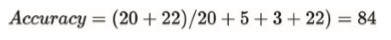
\includegraphics[scale=0.5]{figures/j2b.jpg}
			\caption{Rumus Confusion Matriks}
			\label{contoh}
			\end{figure}
		\item Sehingga dari perhitungan tersebut kita mendapat akurasi 84%.
		\item Berikut adalah gambar klasifikasi biner :
			\begin{figure}[ht]
			\centering
			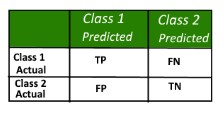
\includegraphics[scale=0.5]{figures/j2c.jpg}
			\caption{Confusion Matriks}
			\label{contoh}
			\end{figure}
	\end{itemize}
	
\item Voting Pada Random Forest
	\begin{itemize}
		\item Voting pada random forest merupakan metode yang paling umum digunakan setelah classifier membuat keputusan.
		\item Gambar voting pada random forest
			\begin{figure}[ht]
			\centering
			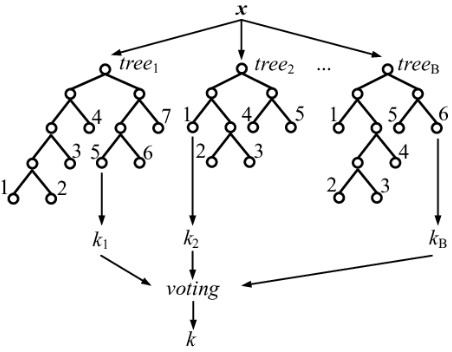
\includegraphics[scale=0.5]{figures/j3.jpg}
			\caption{Voting Pada Random Forest}
			\label{contoh}
			\end{figure}
	\end{itemize}

\end{enumerate}


\section{Method 1}
Definition, steps, algoritm or equation of method 1 and how to apply into your data
\section{Method 2}
Definition, steps, algoritm or equation of method 2 and how to apply into your data